% Typeset by:
%  Will Crawford (wacrawfo@ucsc.edu)

% TODO:
% Most occurrences of ``the algorithm'' should be replaced by ``the scheduler.'' DO NOT do a global find/replace.
% Check on instances of ``he.'' They should probably be changed to ``he/she.''

%%%

% Development Process: Explain the phases of Unified Process.
% Rewrite Scenario 4 and possibly provide a mockup.
% - System should review integrity of schedules, not the administrator. 
% New diagrams around line 200?
% Replace symbols in the diagrams of Requirements: Specification
% Consider removing the old diagrams
% Do we need to mention the fitness function in 4.3: The Algorithm?


%%%%%%%%%%%%%%%%%%%%%%%%%%%%%%%%%%%%%%%%%%%%%%%%%%%%%%%%%%%%%%%%%%%


\documentclass[12pt]{article}
\usepackage{amsmath}
\usepackage{graphicx}
\usepackage{fancyhdr}
\usepackage{array}
\pagestyle{fancy}
\fancyfoot{}
\rfoot{\thepage}

\graphicspath{{./img/}}
\setlength{\parskip}{0.15in}

\title{S.C.O.R.E Report for\\ MyCourses \\ A Course Scheduling System \\ UCSC Team}
\author{Ben Ross \texttt{(bpross@ucsc.edu)} \\
	\and Erik Steggall \texttt{(esteggal@ucsc.edu)}\\
	\and Justin Lazaro \texttt{(jlazaro@ucsc.edu)}\\
	\and Sabba Petri \texttt{(spetri@ucsc.edu)}\\
	\and Will Crawford \texttt{(wacrawfo@ucsc.edu)}}
\date{}

\begin{document}

\maketitle
\pagebreak
\tableofcontents
\pagebreak

\section{Executive Summary}
The MyCourses Scheduler is an end-to-end scheduling system that automates most of the manual labor involved in scheduling university courses. We seek to provide universities an easy-to-use service that can help reduce the costs and complications involved in organizing an entire schedule.


Our team started in mid-September as a group of 5 engineering students taking a ``Software Methodology'' course. We chose to do a course scheduling system as our class project because we felt that the problem was interesting, and that we would learn a lot by writing a system to solve it.

The members of our team are Justin Lazaro, Will Crawford, Ben Ross, Erik Steggall, and Sabba Petri. Our team members have held a variety of roles in the technology industry such as IT, QA, Marketing and System Administration at top technology firms including Hewlett Packard, Riverbed Technologies, and Yahoo!. 


% Review again for tense
\section{Development Process} % Will
\indent This instance of the MyCourses scheduling system was created as part of a class instructed by Professor Linda Werner here at UCSC. Participation in this class required that we approach design very seriously before we started coding. This was a new approach to us as most of our team was accustomed to developing through rapidly iterated prototypes.

After gathering the requirements from the SCORE project description, we immediately discovered that scheduling classes would likely be an NP-hard problem, meaning that there would be no way to find an optimal solution in polynomial time. In other words, it looked like a problem with no canonical ``best answer.'' Much of our time in this phase was spent shopping around for a similar problem whose solution we could apply to our problem. We eventually found a solution in the form of a freely available course scheduling algorithm written by a Serbian software developer named Mladen Jankovic. It was written in C++, so we converted it into Python.

We started out planning our project using the Unified Process, an iterative and incremental software development model. The Unified Process is composed of four phases: inception, elaboration, construction and transition. 

We lacked familiarity with the some of the technologies we planned on using for our project (Django, our Python web framework, in particular). Because of this, we spent much of our inception phase and elaboration phase learning about the functionality and capabilities of these technologies. This allowed us to generate more realistic design documents for our project.

Since this project was being done as part of a class, our instructor required several deliverables from us apart from the requirements of the SCORE project as part of a modified Unified Process. These were primarily presentations and the delivery of documents that we will discuss further in our Project Plan section. 

%% Cut section here %%

% Move below to Project Plan %
For our first deliverable, part of our inception phase, we wrote out scenarios for the use of our product. We included a scenario for each of the user categories that would be using our product. Our Program Administrator scenario described how the Program Administrator would initially set up the database in order to run the algorithm. The scenario for the Program Manager shows how the Program Manager should be able to inspect the courses that the administrator picked, and select the courses and lecturers for the upcoming quarter. The scenario for the lecturer shows how the lecturer should be able to specify their own individual constraints, such as the courses that they wish to teach, and the days and times that they are available. The scenario for the student shows how a student should be able to select a course for their upcoming quarter. We also included a scenario in which the Program Administrator can receive the master schedule from each individual Program Manager and is then able to set up and run the algorithm.

Our second deliverable provided an overview of our requirements, also part of our inception phase. In this deliverable we provided a broad overview of our system and its functionality. It was broken into functionality, performance, usability, constraints, and our wish list. The functionality provides a description of what our system does, we included information on the algorithm, a breakdown of our database, the different sections of our user interface, and the specifications of our server.

Our third deliverable was an overall summary of our project, part of our elaboration phase. We provided a high level architecture that showed the break down of our system into user interface, Django, and the algorithm. We went into detail on how we planned to build our project and reasons for building it the way we did. We also included interaction diagrams, in which we elaborated on the scenarios we selected. 

Our fourth deliverable was a user manual for our project, part of our construction phase. This deliverable was primarily a tutorial for each user role showing how they will use our final product. It had a step-by-step process for setting up accounts and performing the necessary tasks for each role. Our user manual also includes a system overview so that it is more clear for the user reading it.

Our final deliverable was an acceptance test for our project. This deliverable was a working prototype designed to exhibit the same qualities that our final product will have. It demonstrated most of  our project's functionality, though it was far from feature-complete.

\section{Requirements: Problem Statement} % Justin
Scheduling courses is a difficult task for many universities. Manually scheduling hundreds of courses can be very tricky due to limited classroom space, limited professor availability, and limited time to teach these classes. 

We imagine four primary stakeholders for this task: Program Administrators, Program Managers, lecturers, and students. The Program Administrator will be responsible for determining a master list of courses, classrooms and time slots. The Program Managers will select which courses to offer in a given quarter and provide additional information about them such as class size and class location. The lecturers (or professors) will prefer to teach certain courses. They will also prefer to teach at certain times. The students will need to enroll in courses offer in a certain quarter.

\subsection{Scenario}

Below, we outline a common use-case scenario. This scenario was generated along with many others during our inception phase in order to help us understand how users would interact with a system designed to solve this problem. This particular scenario involves a Program Administrator and several Program Managers.

\begin{enumerate}
\item	The Program Administrator signs in to a browser-based system by supplying their credentials to the website.
\item	Once logged in, the Program Administrator is presented with a panel illustrating their privileges - there will be links to pages that let the admin modify the database, add users, etc.
\item	The Program Administrator can click on the database modification link, and will subsequently be presented with its contents in a tabular format.
\item	Choosing to import data, the Program Administrator will need to provide the following: 
	\begin{enumerate}
	\item	A list of all classrooms and buildings available, including...
		\begin{enumerate}	
		\item Room capacity.
		\item Subject preference. (e.g. Social Sciences belong in the Sociology building)
		\end{enumerate}
	\item	A list of all instruction time slots. (e.g. Can classes be taught on Saturday? When are normal instruction hours?)
	\item	A list of courses offered for every subject. 
	\end{enumerate}
\item	The Program Administrator can also manually enter information (e.g. Baskin Engineering $\to$ Room 156 ) or modify imported information. This can be done by clicking on the appropriate element, modifying the appropriate fields, and submitting the changes.
\item	Once the information has been imported and reviewed, each Program Manager can determine which courses will be offered in the upcoming quarter.
\item The Program Manager signs in to the browser-based system by supplying their credentials to the website.
\item The Program Manager sees a message that notifies them that the system has been populated by the Program Administrator for a new quarter. He or she opens a list of all the courses in their department.
\item The Program Manager will select which courses will be offered for this particular quarter.
\item The Program Manager will also specify which instructor will teach each course.
\item After each Program Manager has selected each course to be offered and its corresponding instructor, the Program Administrator will be notified via e-mail.
\item The Program Administrator can then review the entire list of offered courses if he or she chooses. The Program Administrator will also be able to run the scheduler at this point. The scheduler will algorithmically determine when courses will be taught. The system will attempt to provide a best fit and present that to Program Administrator for review, modification, or acceptance.
\end{enumerate}

\section{Requirements: Specification} % Sabba
There are four sections to this system: the user interface, the database, the scheduler, and the connecting component. 

The user interface must be very clean and user-friendly. It must be intuitive both to freshmen students of eighteen and to senior professors of seventy.  

Program Administrators must be able to modify and perform operations on the database. Program Administrators must also be allowed to run the scheduler. They must also have a simple way to communicate with the Program Managers. 

Program Managers must be able to retrieve course information specified by a Program Administrator.  With this information, Program Managers must be able to specify the courses for the upcoming school session. This selection must propagate automatically for the scheduler's usage.

Lecturers must be able to specify preferred teaching times and preferred courses. They must also be able to see which courses they have been selected to teach. This information must be automatically added to the database for the scheduler's usage.

Students must be able to see the scheduler's output once a Program Administrator has accepted it. They must be able to search, view, and select courses from the catalog. As students will traffic the system most heavily, the student's user interface must be especially simple and efficient. 

As students, our team has an advantage in that we are keenly aware of the needs of this particular user role. We are capable of being both designing it from the vantage point of an engineer and testing it from the perspective of a student. 

The database must perform read and write operations efficiently and reliably. It must be robust as potential user bases at some universities are quite large; load on the database will be proportionally large. 

The scheduler must have an algorithm that is first able to handle multiple constraints. This algorithm must be scalable so that, given increasing constraints, it will remain both functional and efficient. If the algorithm cannot find an optimal schedule, it must be able to convey conflicts to Program Administrators and allow them to manually resolve these conflicts.

Lastly, there must be a connecting component that links the user interface, the database, and the scheduler. This connecting component, as with the rest of the system, must be robust under high loads, allowing for both larger and smaller systems.

\begin{enumerate}
\item User Interface
	\begin{enumerate}
	\item The web platform must be:
		\begin{enumerate}
		\item Compatible with multiple browsers.
		\item	Intuitive and easy to understand.
		\end{enumerate}
	\item Views based on user roles:
		\begin{enumerate}
		\item Program Administrators must be able to:
			\begin{enumerate}
		    \item Modify the database.
		    \item Choose constraints for the scheduler.
		    \item Run the scheduler.
		    \end{enumerate}
		\item Program Managers must be able to:
			\begin{enumerate}
		   \item Retrieve information provided by Program Administrator.
		   \item Specify the courses for a certain school session.
		   \end{enumerate}
		\item Lecturers must be able to:
			\begin{enumerate}
			\item Submit preferences to the Program Manager.
			\end{enumerate}
		\item Students must be able to:
			\begin{enumerate}
		   \item Enroll in courses.
		   \end{enumerate}
		\end{enumerate}
	\item Must interact with the connecting component.
	\end{enumerate}
\item Database
	\begin{enumerate}
	\item Must be able to store and retrieve data efficiently and reliably.
	\item Must handle load well.
	\item Must interact with the connecting component.
	\end{enumerate}
\item Scheduler
      \begin{enumerate}
      \item Constraint-based algorithm:
      	    \begin{enumerate}
            \item Must be able to handle multiple constraints (e.g. room capacity, lecturer availability, subject preference, etc.).
	    \item Must be precise in handling schedules for the Program Administrator.
	    \item Must provide an output that is easy to modify, in case the algorithm does not provide a solution for a set of inputs.
	    \end{enumerate}
	\item Must interact with the connecting component.
     \end{enumerate}
\item Connecting Component
      \begin{enumerate}
      \item Must provide an interfacing between the user interface, the database and the scheduler:
    \item Must be robust to allow for systems both small and large.
     \end{enumerate}
\end{enumerate}

\section{Architectural Design} % Erik
Our architecture is broken into four main categories:
\begin{enumerate}
\item User interface or UI (The front end)
\item The database  (The back end)
\item The scheduler (The engine)
\item Django (The framework)
\end{enumerate}

\subsection{The User Interface}
There are four different user interfaces. Each is assigned to one of the four roles that a user could be: Program Administrator, Program Manager, lecturer, and student.

The Program Administrator's user interface is fairly simple. They are given fields to edit elements such as courses, rooms, and professors. Once they fill out the fields for the master list, this list is propagated to the Program Managers. Once the Program Managers have selected course offerings for the quarter or semester, then the Program Administrator may run the scheduler. Once the Program Administrator has accepted the scheduler's output, the schedule will be propagated across the system.

The Program Manager's interface will display all of the courses and lecturers for their department. The Program Manager will have the option of selecting the lecturers and courses that they want to be offered during the quarter or semester.

The lecturer will have an interface that will hold the courses that they can teach and the current courses that they are teaching. They will be able to manually add or drop students from their courses, and assign grades to students in their courses.

The student will have a customizable interface which will hold their past, present and future schedules. It will also have other widgets that they will be able to add to their interface.

\subsection{The Database}
Our database holds several different sets of tables. There is a ``master list`` set of tables that the Program Administrator modifies, and a set of tables that the scheduler outputs to. There are also tables to store individual user data, such as login credentials and course selections. To avoid redundancy, we use foreign keys often in our database.

The master list tables hold the following elements: School, Department, Class, Class lab, Prerequisites, Building, Room, Period, Lecturer, Person, Role, and Person Role.

The scheduler outputs to a set of tables that hold a complete schedule of the quarter or semester. Past schedules will also be stored in the database in the same format. 


\subsection{The Scheduler}
The algorithm we use is a modified genetic algorithm written by Mladen Jankovich, a Serbian software developer. It mimics the process of natural selection in order to find a solution to our scheduling problem. The algorithm represents the variables as ``chromosomes.'' A full set of chromosomes make up a parent. Each parent is given a fitness value according to how well they fit into the schedule. Fitness is higher for matches that fit into empty classrooms, have the appropriate number of seats, or if the classroom has a lab in it. 

A group of parents make up a population. The algorithm takes 'n' number of parents from the population and does a crossover on pairs of the selected parents to create 'n' new chromosomes. The algorithm replaces 'n' chromosomes from the existing population with the new chromosomes that were created by the crossover. It does not replace the chromosomes with the best fitness. After the crossover is performed, mutations take place. A random number is generated, which represents the mutation size. While the size has not been reached, classes are moved to different rooms randomly. Classes with the best fitness are ignored. 

The algorithm repeats this process until it reaches a fitness of one hundred percent. This means it has found a solution that satisfies all of its constraints. The algorithm pulls information from the database, and enters it into four different lists: a professor list, a course list, a room list and a classes list. It then outputs into a second database which is then accessible from the user interface. 

\subsection{Django}
Django connects the user interface, the database and the scheduler. Django manages the user interface by handling the user requests and providing the appropriate response. 

For example, when the scheduler is called by the Program Administrator, the browser creates an HTTP request. Django receives this request and transforms it into an object. It checks the URL and determines to which function it must send the request object. The function in this case is the scheduling algorithm, which takes the information stored in the database and attempts to find a solution. The output of the scheduler is placed into a second database and a response to the request object is generated and sent to the Program Administrator.

% Work the deliverables from Development Process into this section.
\section{Project Plan} % Justin

Our project was part of a software methodology course and many of the deliverables submitted for the class are similar to those in the SCORE requirements. 

Instruction began on September 23, 2010 and continued for ten weeks. Further development of our scheduling system will continue into the Winter quarter whose duration began January 4, 2011 and ends March 18, 2011. 

\subsection*{Week 1: Initial Presentation}

The first week we formed our group and gave an initial presentation on our proposed project. In the presentation we introduced our team's project name and group members, along with an overview of our project. The overview included our desired core functionality, our perceived project risks, our predicted user experience and our wish list. 

\begin{center}\texttt{Perceived Project Risks}\end{center}
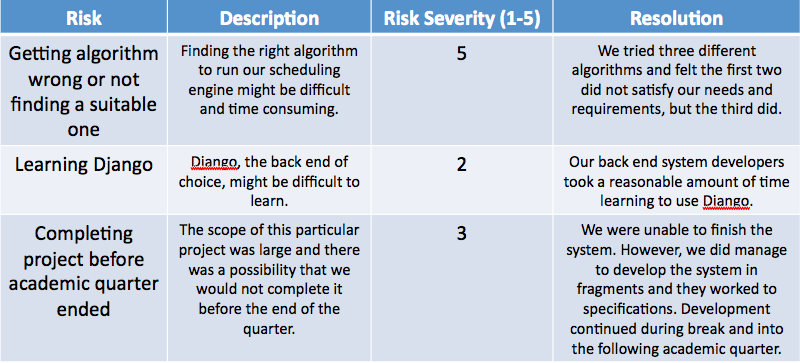
\includegraphics[scale=0.45]{risktable.png}

\subsection*{Week 2: Requirements - Scenarios}

Our team designed user scenarios related to our project. The scenarios were a significant part of our requirements document and were important in defining various aspects of our system's functionality. We came up with user scenarios for the following roles: Program Administrators, Program Managers, lecturers, and students. 

Each scenario outlined and described the flow of data and the interaction with different functions and systems as the user performed a particular action. 

\subsection*{Week 3: Requirements - Complete}

After defining our scenarios, we created a complete requirements document which was necessary for implementing our system. It detailed the specification of the functionality of our scheduler and constraints on that functionality. 

The requirements we described included the following:
\begin{itemize}
\item Functionality - A specific and detailed description and list of our system.
\item Usability - How users would interact with our system.
\item Coding Standards - Rules for organizing and formatting code.
\item Preliminary User Interface - Preliminary mockups of what our user interface would look like. 
\item Wish List - System features we hoped to implement if time permitted.
\end{itemize}

We gave a design presentation which outlined everything in our requirements document and how we planned to do it. 

\subsection*{Week 4: Architecture and Design Document}

After defining our requirements, we created a design document that described the architecture of our system. It had a detailed description of the objects that we would use as well as relationships between objects. 

We included the following items: 
\begin{itemize}
\item Overview - The overview document provided context for our system and an overview of our diagrams. It included descriptions of our major design decisions. 
\item Architecture Diagram - High-level overview of the components in our system and how they co-operate. 
\item UML Structure Diagrams - Diagrams of our class objects that described the attributes and operations in Unified Modeling Language.
\item UML Interaction Diagrams - A diagram that described several of the scenarios we produced for the requirements document. 
\end{itemize}

\subsection*{Week 5-6: Development and User Manual}
During this phase of our course, implementation of our system commenced and continued for the next several weeks. This included implementing our design and requirements document. As we created this system, we simultaneously created a user manual that detailed how our system would work. The user manual explained the user interface  and provided a walkthrough for common tasks.

\subsection*{Week 7: Software Inspection}

Our software inspection was an in-class presentation in which we systematically read source code. We identified and classified defects as we noticed them. For our software inspection, we chose to review our algorithm as it was one of the most difficult parts of our project to debug.

%It is also important to note that a software inspection is strictly a time to catch defects and not make an attempt to discuss how to fix them or what to do to fix. There is no discussion of the problem at this time, it is simply to define the problem and make note of it to the developer. 

\subsection*{Week 8: Unit Test}

Our group created several unit tests using Python, the Django testing suite, and a third-party tool called Selenium. These tested the various modules of our system both separately and in conjunction with one another. 

\subsection*{Week 9-10: Acceptance Test}

With our development, testing, and inspection complete, we demonstrated our system to our professor. 

At this point, the quarter was ending and all our project deliverables were completed and ready to be delivered as a final product. Due to the size of our project, we did not manage to integrate all of its separate modules. However, in isolation, each module worked well. 

Because our system was incomplete at this point, we decided to spend the next academic quarter completing development of our project. The next academic quarter at UC Santa Cruz began January 4, 2011 and would end on March 18, 2011. 

The following is our plan for the second quarter. 

\subsection*{Week 1: Review}

Our plan was to review our system and deliverables. We defined items that remained incomplete or that required improvement. We also discussed switching from the Unified Process to an agile Scrum software development process. We revised our meeting schedule to include short check-ins every night along with a longer weekly planning meeting. 

\subsection*{Week 2: Documentation Development}

At the time of this report's submission, we are at this stage in our plan.

With our SCORE submission approaching, we focus this week on writing the necessary report. After this week concludes, we will continue development on our project.

\subsection*{Week 3-10: Continued Implementation}

During this period, we will return to integrating the disparate modules of our system and adding features from our wish list.

\section{Management Plan} % Erik and Will

\subsection{An Overview of the Management Process}
We chose a democratic team structure; the management is broken into two timeframes corresponding to our schools quarter system. For the first part, of our project we would meet twice a week for a short period of time during our scheduled class time, and at least once outside of class. Meeting often was crucial in coordinating our project early on its development.

For the first quarter, course requirements guided our deliverables and project plan. It took a few weeks for us to settle in our team roles (specified below). For the first few weeks of the project we were all involved in deciding how we were going to structure our system and what needed to be done. We would meet in class and discuss the research everyone had done since our last meeting. We then worked in pairs or individually until our next meeting. We waited until implementation phase to choose specific parts of the project that we would work on. 
 
We revised our management plan at the beginning of the second quarter. We switched to the Scrum process, and we are now meeting once a day for fifteen minutes. Will took over as project manager, and has taken on the responsibility of coordinating our meetings and resolving any issues that prevent team members from making progress. 
	
\begin{description}
\item{\textbf{Ben Ross}} - In charge of coding the algorithm
\item{\textbf{Professor Charlie McDowell}} - Project reviewer
\item{\textbf{Erik Steggall}} - In charge of connecting Django and the scheduler
\item{\textbf{Justin Lazaro}} - In charge of documentation
\item{\textbf{Professor Linda Werner}} - Project reviewer
\item{\textbf{Sabba Petri}} - In charge of the user interface
\item{\textbf{Will Crawford}} - In charge of Django administration and overall expertise
\end{description}

\subsection{Channels of Communication}

\begin{description}
\item{\textbf{Subversion (SVN)}} \\As part of the class, we were required to use Subversion as a project repository for our code. Subversion is a source control mechanism that allows multiple people to remotely collaborate on the same codebase. We used Subversion to transfer code and miscellaneous files between team members. We also used it to automatically merge source code files.
\item{\textbf{Google Groups}} \\For the purposes of communicating by e-mail, we created an e-mail list with Google Groups; it allowed us to automatically archive our e-mail conversations and bounce all communication to each team member. Scheduling meetings was done primarily via this e-mail list. It also initially served as a rudimentary feature tracker.
\item{\textbf{Daily Skype Meetings}} \\After the conclusion of the class, we continued to meet via Skype every night for 15 minutes to check in with each other. These meetings were intended to briefly answer three questions: ``What did you work on today?'' ``What are you working on tomorrow?'' and ``Is there anything preventing you from making progress?''
\item{\textbf{Git \& Codaset}} \\After the class concluded, we switched from Subversion to Git as more of our team members were comfortable with it and preferred it. Git is another source control mechanism, but we found its granularity regarding which files it committed to be superior to that of Subversion. We also found its merging algorithm produced fewer conflicts during our usage. The website Codaset \texttt{(http://codaset.com/)} served as a central repository for the highly mobile team, as well as a GUI for viewing the repository's metadata, such as commit histories, volume, etc.
\end{description}

\section{Implementation} % Ben

The overall system was broken down into four main parts: the web interface, the database, the scheduler, and security. Our implementation strategy was to find the best way to implement these parts separately, and then collectively integrate them together.

The front end of our system was written in HTML and CSS. We picked HTML and CSS because they are the standard web design languages. We decided to use Javascript to add functionality to the front end because it is widely supported and renders much faster than Flash. In addition, unlike Flash, Javascript is rendered in browsers without a plugin.

The Django framework was selected for a few reasons. Django has an interface that allows for robust database operations without as well as a Pythonic template system to display information on dynamic web pages. The use of this framework us to seemlessly integrate the scheduler with the Database. We identified the integration of the scheduler to the Database to be a major risk facing our system development, but was mitigated early in the process. Django uses forms and templates to display information from the database to web pages and this allows us to create a few templates for each of the authentication levels, all of which are able to display information directly from the database with no SQL queries. Because Django performs operations on the database transparently, Python queries are performed with great speed, letting pages load quicker. % Is this last sentence true?

The scheduler was the biggest risk of the development of the system. We choose to implement the scheduler using a genetic algorithm. This Algorithm was based off of a freeware genetic algorithm scheduler[citation goes here]. The Algorithm was written in Python, allowing it to be fast and easily modifiable. The genetic algorithm was selected as the best implementation solution, because it allowed seamless integration with the database, and it proves incredibly fast, even for larger solutions.%Will sent you an email. Not sure on the format for citing. search [citation goes here]

Security is one of the most important aspects of a web application, especially one for universities.Our first important security feature is HTTPS. HTTPS is used because it allows all traffic to be encrypted. The encryption capability is a step above popular web applications like Facebook, and Myspace. Our second important security feature is passwords. Our minimum password length is 8, with a minimum of one capital letter, one symbol, and one letter. This gives users increased security from brute force password attacks. Another security feature involving passwords is similar to what some banks do. We assign each user a sitekey, which is a random picture out of 50. The user is then requested to name the sitekey. When the user enters their password, if an incorrect sitekey is displayed, the user is made aware of an attempt to compromise their information. 

The fourth other security features deal with the privacy of the user once they are in the system. These features are designed for the student role only. The integration of Facebook with our system provided another security hole. When the student first logs into the system, a tutorial walks them through setting up their account and linking it with their Facebook account. The student has the option to turn off sharing of information during this setup, as well as, anytime through the account settings page. This feature gives permission to students for complete access as to what information they share through our system, and through Facebook. Allowing students this control will decrease the chances of a student sharing more information than they intend. %Does Facebook to be need included?

\section{Validation and Verification} % Ben and Erik
Our test framework for our implementation has three forms. Testing for the scheduler, testing for the Web Interface and testing the Database through the Django framework. The testing for the scheduler is done by scripts,the Web Interface testing is done through a software suite, and testing the Database is done through Django's testing suite.

The scheduler was first tested manually by checking the output for a valid schedule. This proved to be very tedious, and long. The Algorithm team developed an automated script that was able to check the schedule, verifying it was valid. The automated script allowed testing of much larger datasets, which helped prove the validity of the scheduler.

The Web Interface testing is done using a framework called Selenium. This open source tool allows automatic testing of the web UI. Two methods were used for writing tests for the web UI. Selenium has an IDE that allows you to record an interaction with the web UI and run that recording as a test. This was done for basic actions, such as logging in and out. The other way our python scripts that use Selenium's built in libraries to interact with the web interface. This allowed us to check for output on a given page. This was done for advanced actions, such as signing up for classes, or adding students to the database.

The Database's testing is done through  Django's test framework.The suite can test the framework with and other utilities. The testing suite is split into two different sections; doctests and unit tests. The tests are run through Python's manager; Python's manager can test the entire Database, or specific modules of it. Our project used the unit test portion of the test suite to test the database and the database to algorithm connection.

\section{Outcomes and Lessons Learned} % All
The development of this project has taught our team many valuable lessons in software development. First, and foremost is learning how to work together as a team to develop a software system. Previous to this project, none of the group members had developed a project of this magnitude. Learning how to divide tasks and break up the work based on skill sets of team members was something that we struggled with at the onset of the project. Because we did not understand the magnitude of the project, we divided tasks based on member's interests of specific tasks. We soon realized this was not the best decision, and our initial development cycle was thrown off because we had to choose roles that we were best suited, even if it was not our first choice.

After using the initial development process for ten weeks, our group decided to change our development process from the Unified Process to Scrum. This decision was made, because our initial process was not suited for the fast paced development that our system needs. The Unified Process had slow increments,the long time delays between due dates allowed members of our group to fall behind on the project. Our new method allows us to keep all members accountable, and to keep everyone updated on the current status of the system. Realizing that one development process does not fit all was a great lesson learned through this project.

Throughout the development of our system, the tools and technologies, that our group was using, were under constant change. Our solution to scheduling changed three times until a suitable solution was found, as a result, there was a lot of time wasted researching technology that was never implemented. Once we were able to utilize our teammember's skills to find the right technology, the development of our project became easier, and was quickly gained speed. The combination of adopting a new development process, locking down the technologies needed, and understanding one another has increased our productivity and our understanding of working on a development team. 

\end{document}

